\documentclass[a4paper]{jsarticle}
\setlength{\topmargin}{-20.4cm}
\setlength{\oddsidemargin}{-10.4mm}
\setlength{\evensidemargin}{-10.4mm}
\setlength{\textwidth}{18cm}
\setlength{\textheight}{26cm}

\usepackage[top=15truemm,bottom=25truemm,left=20truemm,right=20truemm]{geometry}
\usepackage[latin1]{inputenc}
\usepackage{amsmath}
\usepackage{amsfonts}
\usepackage{amssymb}
\usepackage[dvipdfmx]{graphicx}
\usepackage[dvipdfmx]{color}
\usepackage{listings}
\usepackage{listings,jvlisting}
\usepackage{geometry}
\usepackage{framed}
\usepackage{color}
\usepackage[dvipdfmx]{hyperref}
\usepackage{ascmac}
\usepackage{enumerate}
\usepackage{tabularx}
\usepackage{cancel}
\usepackage{scalefnt}

\renewcommand{\figurename}{fig.}
\renewcommand{\tablename}{table }
\newcommand{\redunderline}[1]{\textcolor{BrickRed}{\underline{\textcolor{black}{#1}}}} 

\hypersetup{
	colorlinks=false, % リンクに色をつけない設定
	bookmarks=true, % 以下ブックマークに関する設定
	bookmarksnumbered=true,
	pdfborder={0 0 0},
	bookmarkstype=toc
}

\lstset{
basicstyle={\ttfamily},
identifierstyle={\small},
commentstyle={\smallitshape},
keywordstyle={\small\bfseries},
ndkeywordstyle={\small},
stringstyle={\small\ttfamily},
frame={tb},
breaklines=true,
columns=[l]{fullflexible},
xrightmargin=0zw,
xleftmargin=3zw,
numberstyle={\scriptsize},
stepnumber=1,
numbersep=1zw,
lineskip=-0.5ex
}

\setcounter{tocdepth}{3}

\author{}
\title{流体力学}
\date{}

\begin{document}
\maketitle
% \tableofcontents
% \newpage

\section{静止流体の力学}
\subsection{静水圧}
静止している液体の任意の点にはたらく圧力のことを\textgt{静水圧}(水圧)という.
流体内の任意の1点における圧力は,\textgt{すべての方向に対して等しい}.
\subsection{(例題) 流入出口が受ける圧力}
\begin{figure}[htbp]
    \begin{center}
        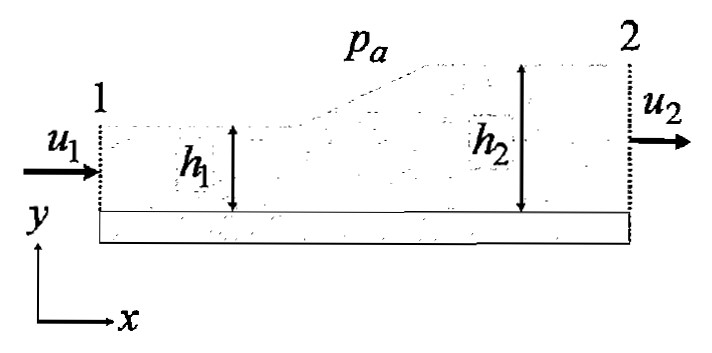
\includegraphics[width=120mm]{images/ryuriki_image4.jpg}
        \caption{H21 試験問題[7]}
    \end{center}
\end{figure}
流入出口に加わる外からの力$F_1,F_2$を求める.ただし,液体の密度は$\rho$,重力加速度を$g$とする.
\begin{enumerate}[(1)]
    \item \textgt{断面1に加わる力$F_1$}\\
          板の上面を$y=0$として,発生する圧力$P_1\left(y\right)$は
          \begin{eqnarray*}
              P_1\left(y\right)=\rho g \left(h_1-y\right)
          \end{eqnarray*}
          と表せるので,断面1に加わる力$F_1$は,
          \begin{eqnarray*}
              F_1=\int_0^{h_1} P_1\left(y\right)dy =\rho g \left[h_1y - \frac{1}{2}y^2\right]_0^{h_1} = \frac{1}{2}\rho g h_1^2
          \end{eqnarray*}
    \item \textgt{断面2に加わる力$F_2$}\\
          同様に,板の上面を$y=0$として,発生する圧力$P_2\left(y\right)$は
          \begin{eqnarray*}
              P_2\left(y\right)=\rho g \left(h_2-y\right)
          \end{eqnarray*}
          と表せるので,断面1に加わる力$F_2$は,
          \begin{eqnarray*}
              F_2=\int_0^{h_2} P_2\left(y\right)dy =\rho g \left[h_2y - \frac{1}{2}y^2\right]_0^{h_2} = \frac{1}{2}\rho g h_2^2
          \end{eqnarray*}
\end{enumerate}
したがって,求める力$F_1,F_2$は以下のようになる.
\begin{eqnarray*}
    \begin{cases}
        F_1= \dfrac{1}{2}\rho g h_1^2 \\
        \\
        F_2= \dfrac{1}{2}\rho g h_2^2 \\
    \end{cases}
\end{eqnarray*}
\subsection{表面張力}
液体の分子間には引張合う力がはたらいており,気体やほかの液体と接している面には縮もうとする力が作用する.
これを\textgt{表面張力}といい,単位は$\left[\mathrm{N/m}\right]$である.
\begin{itembox}[l]{Point}
    \begin{center}
        上下方向の力のつり合いを考える\\
    \end{center}
\end{itembox}
\begin{itembox}[l]{表面張力}
    \begin{center}
        表面張力は,\textgt{境界面の接線方向}にはたらく\\
        ( \textgt{液体の重量$\left[\mathrm{N}\right]$} ) = ( \textgt{表面張力の垂直方向成分$\left[\mathrm{N/m}\right]$}) $\times$ ( \textgt{境界面の周の長さ}$\;\left[\mathrm{m}\right]$ )
    \end{center}
\end{itembox}
\section{粘性流体の力学}
流体の運動における未知量は,\textgt{速度,圧力,密度,温度}である.\\
また,\textgt{時間$\left(t\right)$,空間$\left(x,y,z\right)$}の関数である.\\
\begin{itembox}[l]{Point}
    \begin{eqnarray*}
        (圧縮性流体)&&\quad 未知量は4つ\quad 速度\left(u,v,w\right),圧力\left(p\right)\\
        (非圧縮性流体)&&\quad 未知量は6つ\quad 速度\left(u,v,w\right),圧力\left(p\right),密度\left(\rho\right),温度\left(T\right)\\
    \end{eqnarray*}
\end{itembox}
\section{流体の質量保存則}
\begin{itembox}[l]{連続の式}
    \begin{eqnarray*}
        \dfrac{\partial\rho}{\partial t}+\dfrac{\partial \left(\rho u\right)}{\partial x}+\dfrac{\partial \left(\rho v\right)}{\partial y}+\dfrac{\partial \left(\rho w\right)}{\partial z}&=&0\quad(3次元)\\
        \dfrac{\partial\rho}{\partial t}+\dfrac{\partial \left(\rho u\right)}{\partial x}+\dfrac{\partial \left(\rho v\right)}{\partial y}&=&0\quad(2次元)\\
    \end{eqnarray*}
\end{itembox}
\section{流体のエネルギー保存則}
\begin{itembox}[l]{Point}
    \begin{center}
        流線を意識して、つり合いの式を立てる
    \end{center}
\end{itembox}
完全流体(非粘性・非圧縮性)の定常流れにおいて、任意の流れに沿って、
圧力・運動エネルギ・ポテンシャルエネルギの総和が流線ごとに保存されることを示している以下の式を\textgt{ベルヌーイの定理}という.
\begin{itembox}[l]{ベルヌーイの定理}
    \begin{eqnarray*}
        \dfrac{1}{2}v^2+\dfrac{p}{\rho}+gz=const\\
    \end{eqnarray*}
\end{itembox}
※ ベルヌーイの定理では、単位質量流量あたりのエネルギーの総和を考える.\\
また、水平な流れでは、ポテンシャルエネルギの項を省略して、
\begin{itembox}[l]{水平な流れのベルヌーイの定理}
    \begin{eqnarray*}
        p+\frac{1}{2}\rho u^2 =p_0\\
    \end{eqnarray*}
\end{itembox}
ここで、$p$を\textgt{静圧}、$\dfrac{1}{2}\rho u^2$を\textgt{動圧}、$p_0$を\textgt{総圧(全圧)}という.\\
流れがせき止められ、流速がゼロになる点を\textgt{よどみ点}という。また、$p_0$はよどみ点圧力でもある。\\
※ ベルヌーイの定理は,\textgt{エネルギー保存則}であるのでエネルギーの損失 (圧力損失 等) がある場合は適用できない\\
→ 運動量保存則が適用される\\
\subsection{トリチェリの定理}
容器に液体を入れ,容器に対して十分に小さい穴をあける.
このとき,流れが定常であるとすると,流れ出す液体の速度$v$は以下のように表される.
\begin{itembox}[l]{トリチェリの定理}
    \begin{eqnarray*}
        v&=&\sqrt{2gh}\\
        g&:&重力加速度\\
        h&:&水面から穴までの高さ\\
    \end{eqnarray*}
\end{itembox}
これは,ベルヌーイの定理を用いることで証明できる.
\section{流体の運動量保存の法則}
\begin{itembox}[l]{Point}
    \begin{center}
        \textgt{検査領域}に対する方向に正負をを定める\\
        \textgt{(流入側に加わる力) + (流入側の運動量) = (流出口に加わる力) + (流出側の運動量)}
    \end{center}
\end{itembox}
\begin{itembox}[l]{運動量保存則}
    \begin{eqnarray*}
        \displaystyle\sum mv=Ft
    \end{eqnarray*}
    両辺を時間$t$で微分すると,
    \begin{eqnarray*}
        \displaystyle\sum \dot{m}v=F\\
    \end{eqnarray*}
\end{itembox}
\section{(例題) 運動量保存則}
\begin{figure}[htbp]
    \begin{center}
        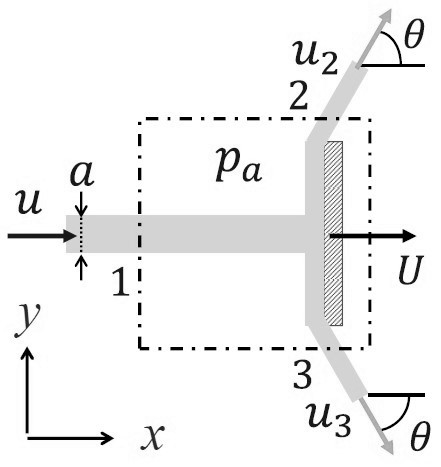
\includegraphics[width=80mm]{images/ryuriki_image5.jpg}
        \caption{流体力学1 演習問題}
    \end{center}
\end{figure}
・平板に加わる$x$方向の力を求める\\
流体の流入速度は
\begin{eqnarray*}
    u'=u-U
\end{eqnarray*}
また、ベルヌーイの定理より、
\begin{eqnarray*}
    \frac{P_a}{\rho}+\frac{1}{2}{u'}^2+\frac{P_a}{\rho}+\frac{1}{2}{u'}_2^2+\frac{P_a}{\rho}+\frac{1}{2}{u'}_3^2
\end{eqnarray*}
したがって、
\begin{eqnarray*}
    u'={u'}_2={u'}_3
\end{eqnarray*}
また、連続の式より、
\begin{eqnarray*}
    \rho {u'} a= \rho {u'}_2 a_2 + \rho {u'}_3 a_3
\end{eqnarray*}
流れの対象性より、$a_2 = a_3$であるので、
\begin{eqnarray*}
    \frac{1}{2}\rho {u'} a = \rho {u'}_2 a_2 = \rho {u'}_3 a_3
\end{eqnarray*}
ここで、断面積2を通過する流体の$x$方向の運動量$\dot{p_2}$は
\begin{eqnarray*}
    \dot{p_2}&=&\rho {u'}_2 a_2 \times {u'}\cos\theta\\
    &=&\frac{1}{2} \rho {u'}^2 a\cos\theta
\end{eqnarray*}
流体が物体に及ぼす$x$方向の力を$F_x$とすると、
\begin{eqnarray*}
    F_x&=&\rho {u'}^2 a - 2 \times \frac{1}{2} \rho {u'}^2 a\cos\theta\\
    &=&\rho {u'}^2 a \left(1-\cos \theta\right)\\
    &=&\rho \left(u-U\right)^2 a \left(1-\cos \theta\right)\\
\end{eqnarray*}
\section{流体の運動方程式}
\subsection{流体の運動を表す2つの運動方程式}
\begin{itembox}[l]{オイラーの運動方程式(2次元)}
    \begin{eqnarray*}
        \dfrac{\partial u}{\partial t}+u\dfrac{\partial u}{\partial x}+v\dfrac{\partial u}{\partial y}&=&-\dfrac{1}{\rho}\dfrac{\partial p}{\partial x}+f_x\quad(x方向)\\
        \dfrac{\partial v}{\partial t}+u\dfrac{\partial v}{\partial x}+v\dfrac{\partial v}{\partial y}&=&-\dfrac{1}{\rho}\dfrac{\partial p}{\partial x}+f_y\quad(y方向)\\
    \end{eqnarray*}
\end{itembox}
\begin{itembox}[l]{ナビエ・ストークス方程式(2次元)\quad(非圧縮性流体)}
    \begin{eqnarray*}
        \dfrac{\partial u}{\partial t}+u\dfrac{\partial u}{\partial x}+v\dfrac{\partial u}{\partial y}&=&-\dfrac{1}{\rho}\dfrac{\partial p}{\partial x}+\nu\left(\dfrac{\partial^2 u}{\partial x^2}+\dfrac{\partial^2 u}{\partial y^2}\right)+f_x\quad(x方向)\\
        \dfrac{\partial v}{\partial t}+u\dfrac{\partial v}{\partial x}+v\dfrac{\partial v}{\partial y}&=&-\dfrac{1}{\rho}\dfrac{\partial p}{\partial y}+\nu\left(\dfrac{\partial^2 v}{\partial x^2}+\dfrac{\partial^2 v}{\partial y^2}\right)+f_y\quad(y方向)\\
        ※\quad \nu &=& \frac{\mu}{\rho} \;:\; 動粘性係数\\
    \end{eqnarray*}
\end{itembox}
\begin{itembox}[l]{ナビエ・ストークス方程式の境界条件}
    \begin{enumerate}
        \item 定常流れ
              \begin{eqnarray*}
                  \dfrac{\partial u}{\partial t}=0
              \end{eqnarray*}
        \item 完全に発達した流れ
              \begin{eqnarray*}
                  \dfrac{\partial u}{\partial x}=0
              \end{eqnarray*}
    \end{enumerate}
\end{itembox}
\begin{itembox}[l]{極座標系の支配方程式\quad(非圧縮性流体)}
    \begin{eqnarray*}
        \dfrac{1}{r}\dfrac{\partial \left(rv_r\right)}{\partial r}+\dfrac{1}{r}\dfrac{\partial v_\theta}{\partial \theta}=0\quad&&(連続の式)\\
        \dfrac{\partial v_r}{\partial t}+v_r\dfrac{\partial v_r}{\partial r}+\dfrac{v_\theta}{r}\dfrac{\partial v_r}{\partial \theta}-\dfrac{{v_\theta}^2}{r}=-\dfrac{1}{\rho}\dfrac{\partial p}{\partial r}+\nu \left(\dfrac{\partial^2 v_r}{\partial r^2}+\dfrac{1}{r}\dfrac{\partial v_r}{\partial r}+\dfrac{1}{r^2}\dfrac{\partial^2 v_r}{\partial \theta^2}-\dfrac{v_r}{r^2}-\dfrac{2}{r^2}\dfrac{\partial v_\theta}{\partial \theta}\right)+f_r\quad&&(r方向)\\
        \dfrac{\partial v_\theta}{\partial t}+v_r\dfrac{\partial v_\theta}{\partial r}+\dfrac{v_\theta}{r}\dfrac{\partial v_\theta}{\partial \theta}+\dfrac{v_rv_\theta}{r}=-\dfrac{1}{\rho}\dfrac{1}{r}\dfrac{\partial p}{\partial \theta}+\nu\left(\dfrac{\partial^2 v_\theta}{\partial \theta^2}+\dfrac{1}{r}\dfrac{\partial v_\theta}{\partial r}+\dfrac{1}{r^2}\dfrac{\partial^2 v_\theta}{\partial \theta^2}-\dfrac{v_\theta}{r^2}+\dfrac{2}{r^2}\dfrac{\partial v_r}{\partial \theta}\right)+f_\theta\quad&&(\theta 方向)\\
    \end{eqnarray*}
\end{itembox}
\subsection{オイラーの運動方程式とナビエ・ストークス方程式の違い}
2つの方程式を見比べてみると,オイラーの運動方程式はナビエ・ストークス方程式から\textgt{粘性項}を除いたものとなっている.
したがって,オイラーの運動方程式では,流体の粘性について考慮されていないことになる.\\
オイラーの運動方程式に従った簡単な例を挙げると,自動車の走行中に流体から力(空気抵抗)を受けないことになる.(実際は抵抗を受ける)\\
また,このパラドクスのことを\textgt{ダランベールの背理}という.そこで,このパラドクスを解くために考え出されたのが,\textgt{ナビエ・ストークス方程式}である.\\
※ オイラーの運動方程式に支配される流体を\textgt{完全流体}という.\\
※ ナビエ・ストークス方程式に支配される流体を\textgt{ニュートン流体}という.(粘性によるせん断応力と速度勾配が比例関係になるような流体)

\section{2次元の連続の式・オイラーの運動方程式の導出}
\begin{figure}[htbp]
    \begin{center}
        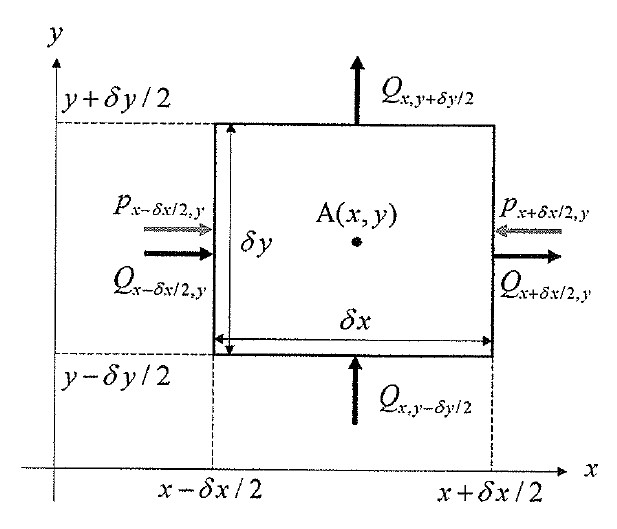
\includegraphics[width=120mm]{images/ryuriki_image1.jpg}
        \caption{R3 試験問題[7]}
    \end{center}
\end{figure}
\subsection{2次元の連続の式の導出}
\begin{itembox}[l]{Point}
    \begin{center}
        時刻$t-\delta t/2\leq t \leq t+\delta t/2$の微小時間$\delta t$間の流れについて\textgt{空間}・\textgt{時間}の観点から保存則を立てる
    \end{center}
\end{itembox}
図1において,連続の式を導出する.
\noindent$\delta t$間に流入する流体の質量を$M_{in}$,$\delta t$間に流出する流体の質量を$M_{out}$,$\delta t$間の質量増加量を$\Delta M$とすると,\\
・\textgt{流入・流出量(空間的観点)}
\begin{eqnarray*}
    M_{in}&=&\left(\rho u\right)_{x-\frac{1}{2}\delta x}\delta y \delta t+\left(\rho v\right)_{y-\frac{1}{2}\delta y}\delta x \delta t\\
    M_{out}&=&\left(\rho u\right)_{x+\frac{1}{2}\delta x}\delta y \delta t+\left(\rho v\right)_{y+\frac{1}{2}\delta y}\delta x \delta t\\
\end{eqnarray*}
\noindent
・\textgt{質量増加量(時間的観点)}
\begin{eqnarray*}
    \Delta M=\left(\rho\right)_{t+\frac{1}{2}\delta t}\delta x \delta y-\left(\rho\right)_{t-\frac{1}{2}\delta t}\delta x \delta y
\end{eqnarray*}
質量保存則より,
\begin{eqnarray*}
    (質量増加量)&=&(流入量)-(流出量)\\
    \Delta M&=&\quad M_{in}\quad -\quad M_{out}\\
\end{eqnarray*}
※ 「増加量」は「流入量」$\geq$「流出量」のときに増加する\\
\\
ここで,$\delta x, \delta y, \delta t$のオーダまでTaylor級数展開すると\\
\\
※ ここでは,点$(x,y)$周りの$\left(x,y\right)=\left(x\pm \frac{\delta x}{2},y\pm \frac{\delta y}{2}\right)$のときについて考えている.
\begin{eqnarray*}
    \left(\rho u\right)_{x\pm \frac{1}{2}\delta x}&=&\rho u\pm \frac{\delta x}{2}\frac{\partial\left(\rho u\right)}{\partial x}+O\left(\delta x^2\right)\\
    \left(\rho v\right)_{y\pm \frac{1}{2}\delta y}&=&\rho v\pm \frac{\delta y}{2}\frac{\partial\left(\rho v\right)}{\partial y}+O\left(\delta y^2\right)\\
    \left(\rho\right)_{t\pm \frac{1}{2}\delta t}&=&\rho \pm \frac{\delta t}{2}\frac{\partial \rho}{\partial t}+O\left(\delta t^2\right)
\end{eqnarray*}
したがって,上式を代入すると,
\begin{eqnarray*}
    \dfrac{\partial \rho}{\partial t}\delta x \delta y \delta t&=&-\left(\frac{\partial\left(\rho u\right)}{\partial x}+\frac{\partial\left(\rho v\right)}{\partial y}\right)\delta x \delta y \delta t\\
\end{eqnarray*}
これを変形して,
\begin{eqnarray*}
    \dfrac{\partial p}{\partial t}+\frac{\partial\left(\rho u\right)}{\partial x}+\frac{\partial\left(\rho v\right)}{\partial y}&=&0
\end{eqnarray*}
以上より,2次元空間における連続の式を導くことができた.
\subsection{2次元のオイラーの運動方程式の導出 (未完成)}
\subsection{クエット流}
2枚の平行な板の間に流体を満たし、一方の板を平行に動かしたときに生じる流れのことを\textgt{クエット流}という.
\begin{itembox}[l]{クエット流}
    \begin{eqnarray*}
        u\left(y\right)&=&\frac{U}{h}y\\
        U \;&:&\; 板の動く速度\\
        h \;&:&\; 板間の距離\\
    \end{eqnarray*}
\end{itembox}
\subsection{ハーゲン・ポアズイユ流}
断面積が一定の円管内をゆっくりと流れる流れのことを\textgt{ハーゲン・ポアズイユ流}という.
\begin{itembox}[l]{ハーゲン・ポアズイユ流}
    \begin{eqnarray*}
        u\left(r\right)&=&-\frac{1}{4\mu}\left(\frac{dp}{dx}\right)\left(r_0^2-r^2\right)\\
        r_0\; &:&\; 円管の半径\\
    \end{eqnarray*}
\end{itembox}
\section{流体のせん断応力}
流体の流れに平行な軸を$x$軸,垂直な軸を$y$とすると,せん断応力$\tau\left(y\right)$は以下のように表せる.
\begin{itembox}[l]{せん断応力(2次元)}
    \begin{eqnarray*}
        \tau\left(y\right)=\mu\dfrac{du}{dy}\\
    \end{eqnarray*}
\end{itembox}

\subsection{(例題) 板が流体から受ける力}
\begin{itembox}[l]{Point}
    \begin{center}
        \textgt{下の物体}が,\textgt{上の物体}から受ける力
    \end{center}
\end{itembox}
\begin{figure}[htbp]
    \begin{center}
        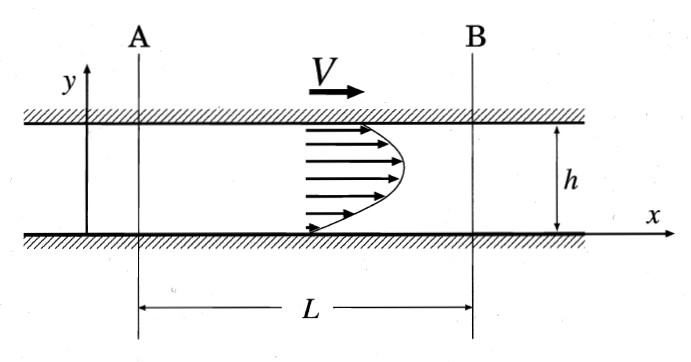
\includegraphics[width=120mm]{images/ryuriki_image3.jpg}
        \caption{H20 試験問題[8]}
    \end{center}
\end{figure}
\\
A-B間の下側の板と上側の板が受ける力$F_1,F_2$を求める.\\
ただし,奥行方向は単位長さとして,流速$u\left(y\right)$は以下のように定める.
\begin{eqnarray*}
    u\left(y\right)&=&-\frac{1}{2\mu}\frac{dP}{dx}\left(h-y\right)y+\dfrac{V}{h}y\\
\end{eqnarray*}
また,このときのせん断力$\tau \left(y\right)$は,以下のように求められる.
\begin{eqnarray*}
    \tau \left(y\right) = \mu \frac{du}{dy} = -\frac{1}{2}\frac{dP}{dx}\left(h-2y\right)+\mu\frac{V}{h}\\
\end{eqnarray*}
A-B間の面積$S$は,以下のように求められる.
\begin{eqnarray*}
    S=L\times 1 =L\\
\end{eqnarray*}
\begin{enumerate}[(1)]
    \item A-B間の下側の板に加わる力を求める\\
          \begin{eqnarray*}
              F_1&=&\tau\left(0\right)\times S\\
              &=&-\frac{hL}{2}\frac{dP}{dx}+\mu\frac{VL}{h}\\
          \end{eqnarray*}
    \item A-B間の上側の板に加わる力を求める\\
          \begin{eqnarray*}
              F&=&\tau\left(h\right)\times S\\
              &=&\frac{hL}{2}\frac{dP}{dx}+\mu\frac{VL}{h}\\
          \end{eqnarray*}
          このとき,上記の力$F$は\textgt{流体が上の板から受ける力}を表しているため,
          上の板が流体から受ける力$F_2$は,
          \begin{eqnarray*}
              F_2&=&-F\\
              &=&-\frac{hL}{2}\frac{dP}{dx}-\mu\frac{VL}{h}\\
          \end{eqnarray*}
\end{enumerate}
したがって,求める$F_1,F_2$は以下のようになる.
\begin{eqnarray*}
    \begin{cases}
        F_1=-\dfrac{hL}{2}\dfrac{dP}{dx}+\mu\dfrac{VL}{h} \\
        \\
        F_2=-\dfrac{hL}{2}\dfrac{dP}{dx}-\mu\dfrac{VL}{h} \\
    \end{cases}
\end{eqnarray*}
\section{応力テンソル}
\begin{itembox}[l]{二次元非圧縮流体における応力テンソル}
    \begin{eqnarray*}
        \sigma_{ij}=-\delta_{ij}P+\mu\left(\frac{\partial u_i}{\partial x_j}+\frac{\partial u_j}{\partial x_i}\right)\\
    \end{eqnarray*}
\end{itembox}
\begin{itembox}[l]{それぞれの応力成分}
    \begin{eqnarray*}
        \sigma_{xx} &=& -P+2\mu\left(\frac{\partial u}{\partial x}\right)\\
        \sigma_{yy} &=& -P+2\left(\frac{\partial v}{\partial y}\right)\\
        \sigma_{xy} &=& \mu\left(\frac{\partial u}{\partial y}+\frac{\partial v}{\partial x}\right)\\
        \sigma_{yx} &=& \mu\left(\frac{\partial v}{\partial x}+\frac{\partial u}{\partial y}\right)\\
    \end{eqnarray*}
\end{itembox}
\section{レイノルズ数}
\textgt{慣性力}と\textgt{粘性力}の比をとった無次元数のことを\textgt{レイノルズ数}という.\\
分母が粘性力,分子が慣性力を表しており,粘性力が支配的な流れは\textgt{層流},慣性力が支配的となる流れは\textgt{乱流}となる.\\
\begin{itembox}[l]{レイノルズ数}
    \begin{eqnarray*}
        \mathrm{Re}&=&\dfrac{UL}{\nu}\\
        \mathrm{Re} &:& レイノルズ数\\
        U &:& 代表速度\\
        L &:& 代表長さ\\
        \nu &:& 動粘性係数\\
    \end{eqnarray*}
\end{itembox}
\section{境界層}
\begin{itembox}[l]{境界層}
    \begin{center}
        粘性の影響を無視できない領域のことを\textgt{境界層}という.\\
        境界層内 : \textgt{粘性流}として扱う  \\
        境界層外 : \textgt{非粘性流}として扱う
    \end{center}
\end{itembox}
\begin{itembox}[l]{剥離点}
    \begin{center}
        流体が原則され続けることで逆流が生じることを,\textgt{剥離}という.\\
        また,剥離が生じる点(位置)を\textgt{剥離点}という.\\
        剥離点は以下の式を満たす.
    \end{center}
    \begin{eqnarray*}
        \left(\frac{\partial u}{\partial y}\right)_{y\neq 0}=0\\
    \end{eqnarray*}
\end{itembox}
\section{流れ場の幾何学的表現}
流れ場を表現する手法として\textgt{流線}・\textgt{流跡線}・\textgt{流脈線}という概念がある.\\
\subsection{流線}
流線は,時間$t$をある時刻に固定し,その時刻における速度ベクトルが接線ベクトルとなる曲線のことである.\\
つまり,$\vec{u}\parallel d\vec{x}$が成立する.
\begin{itembox}[l]{流線}
    \begin{eqnarray*}
        \dfrac{dx}{u}&=&\dfrac{dy}{v}=\dfrac{dz}{w}\\
        vdx&-&udy=0\quad (2次元)\\
    \end{eqnarray*}
\end{itembox}
流線が交差するとき,その交点では流体は速度ゼロもしくは無限大をとる.
速度がゼロのとき,その交点を\textgt{よどみ点}といい,無限大のとき\textgt{特異点}という.
また,この流線によって作られる曲面を\textgt{流管}という.
\subsection{流跡線}
流跡線は,流体粒子を時間とともにラグランジュ的に追跡したときに描かれる軌跡を示す概念であり,以下のように表される.
\begin{itembox}[l]{流跡線}
    \begin{eqnarray*}
        d\vec{x}=\vec{u}dt\\
    \end{eqnarray*}
\end{itembox}
\subsection{流脈}
空間のある点を通過した流体のすべての粒子が任意の瞬間に存在する点を結んだ線のこと.\\
例) たばこの煙をある瞬間に撮影したもの
\section{渦度}
流れ場の回転の程度を表す量を\textgt{渦度}という.
$\vec{u}=\left(u,v\right)$のとき,以下のように表される.
\begin{itembox}[l]{渦度}
    \begin{eqnarray*}
        \zeta = rot\;\vec{u}=\dfrac{\partial v}{\partial x}-\dfrac{\partial u}{\partial y}\\
    \end{eqnarray*}
\end{itembox}
また,渦度$\zeta$は回転の角速度$\omega$の2倍に等しい.
\begin{eqnarray*}
    \omega = \dfrac{1}{2}\zeta\\
\end{eqnarray*}
ここで,$\zeta=0$のとき,回転のない運動(\textgt{渦なし流れ})となる.これを\textgt{ポテンシャル流}という.
\section{流れ関数}
以下の条件を満たす関数$\psi$を\textgt{流れ関数}という.
\begin{itembox}[l]{流れ関数}
    \begin{eqnarray*}
        u=\dfrac{\partial \psi}{\partial y}\quad v=-\dfrac{\partial \psi}{\partial x}\\
    \end{eqnarray*}
\end{itembox}
$\psi =const$のとき,全微分をとると\\
\begin{eqnarray*}
    d\psi = \dfrac{\partial \psi}{\partial x}dx+\dfrac{\partial \psi}{\partial y}dy=0\\
\end{eqnarray*}
これは,流線の定義と同じになっていることがわかる.すなわち,$\psi = const$は流線を表す.\\
※ 流線と関係が深い → 流れの方向ベクトルを表すことができる.
\section{速度ポテンシャル}
以下の条件を満たす関数$\phi$を\textgt{速度ポテンシャル}という.
また,このとき流れは\textgt{渦なし流れ}である必要がある.
\begin{itembox}[l]{速度ポテンシャル}
    \begin{eqnarray*}
        u=\dfrac{\partial \phi}{\partial x}\quad v=\dfrac{\partial \phi}{\partial y}\\
    \end{eqnarray*}
\end{itembox}
速度ポテンシャル$\phi = const$の曲線を\textgt{等ポテンシャル線}と呼ぶ.\\
※ 渦度$\zeta$と関係が深い → 流れに渦(回転運動)がない状態のことを表すことができる
\section{コーシー・リーマンの関係式}
\textgt{定常かつ渦なし流れ}のとき,以下の関係(\textgt{コーシー・リーマンの関係式})が成立する.
\begin{itembox}[l]{コーシー・リーマンの関係式}
    \begin{eqnarray*}
        u&=&\dfrac{\partial \phi}{\partial x}=\dfrac{\partial \psi}{\partial y}\\
        v&=&\dfrac{\partial \phi}{\partial y}=-\dfrac{\partial \psi}{\partial x}\\
    \end{eqnarray*}
\end{itembox}
これは,$\phi$と$\psi$の直交性を示す.
すなわち,流線($\psi=zconst$)と等ポテンシャル線($\phi=const$)は直交する.
\subsection{直交性の証明}
コーシー・リーマンの関係式が成立するとき,
$\psi=const\quad \phi=const$の法線ベクトルはそれぞれ,
\begin{eqnarray*}
    grad \psi&=&\left(\dfrac{\partial \psi}{\partial x}, \dfrac{\partial \psi}{\partial y}\right)\\
    grad \phi&=&\left(\dfrac{\partial \phi}{\partial x}, \dfrac{\partial \phi}{\partial y}\right)
\end{eqnarray*}
これらの内積を計算すると,
\begin{eqnarray*}
    grad\psi \cdot grad\phi &=& \dfrac{\partial \psi}{\partial x}\dfrac{\partial \phi}{\partial x} +\dfrac{\partial \psi}{\partial y}\dfrac{\partial \phi}{\partial y}\\
    &=&\dfrac{\partial \phi}{\partial x}\left(-\dfrac{\partial \phi}{\partial y}\right)+\dfrac{\partial \phi}{\partial y}\dfrac{\partial \phi}{\partial x}\\
    &=&0
\end{eqnarray*}
したがって,2つの法線ベクトルは直行しているといえる.よって,流れ関数$\psi$と速度ポテンシャル$\phi$の直交性は示された.

\end{document}